  \subsection{Group Research}


\begin{table}[H]
	\centering
    
    \begin{tabular}{|p{3.5cm}|p{10.3cm}|}
    
    \hline
    \textbf{\large{Actors}}  			& \tabitem Third Party 																\\
    \hline
    \textbf{\large{Goals}} 				&
    \ref{goal:parties3};
    \ref{goal:parties4};
    \ref{goal:parties5}
    \\
    
    \hline
    \textbf{\large{Enter Condition}}	& The \emph{Third Party} is already logged in	\\
    
    \hline
    \textbf{\large{Events Flow}}		& \begin{enumerate}[leftmargin=0.5cm]
                                \item The \emph{Third Party} selects the Group section
                                \item The \emph{Third Party} selects the "New Request" button
                                \item The \emph{Third Party} specifies the group constraints (such as city or location, the age interval, gender, height and weight, that can be chosen optionally)
                                 \item The \emph{Third Party} selects the data that wants to retrieve and, if it has chosen the subscription mode, should also specify the interval time for the updates
                                 \item Finally, the \emph{Third Party} sends the request, selecting the "Send" button
                                 \item If the privacy constraints are respected, the \emph{System} sends the requested anonymous data to the \emph{Third Party}
                                           
                                          \end{enumerate}
    										\\
    \hline
    \textbf{\large{Exit Condition}} 	& The System shows the                                     anonymized data relative to the                                    \emph{Third Party} specifications. \\
    
    \hline
    \textbf{\large{Exception}} 			& \begin{enumerate}[leftmargin=0.5cm] \item The \emph{Third                                       Party} specified an inexistent city or                                 location.
                                 \item The \emph{Third Party} specified an impossible age/height/weight range.  \item In subscription mode, the \emph{Third Party} hasn't specified an update interval time
                                 \item The \emph{Third Party} hasn't specified the data that wants to retrieve
    \end{enumerate}
    										If one of these problems occur, the System shows a error message to the Third Party, which is invited to re-insert the data or to specify the missing data.
    							
    							\\
    
    \hline
    
    
    \end{tabular}
	
\end{table}
\begin{figure}[H]
    \centering
    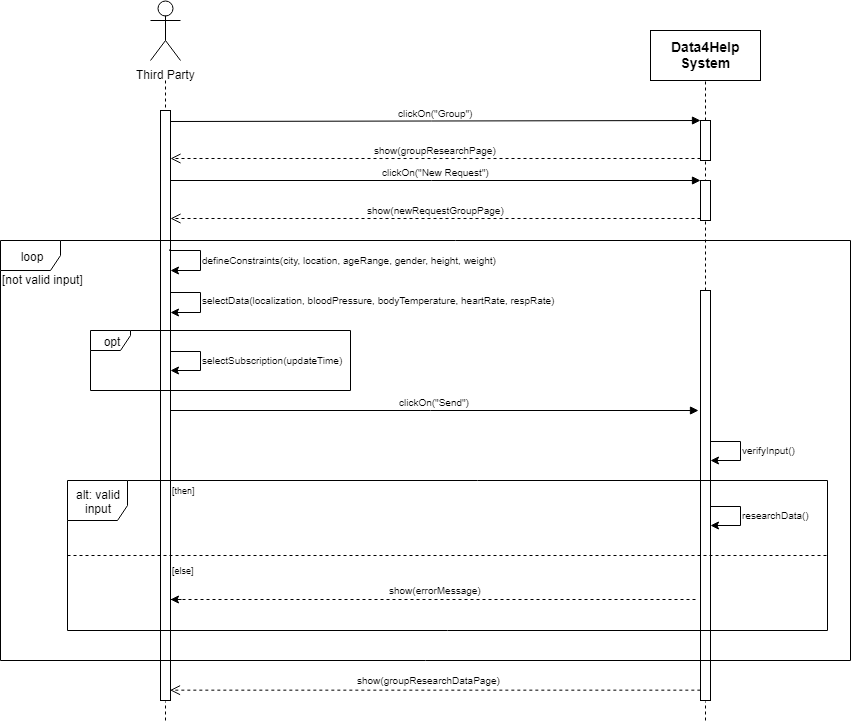
\includegraphics[scale=0.4]{rasdL/Pictures/groupResearchSeqDiag.png}
    
\end{figure}
